\documentclass[10pt,a4paper]{article}
\usepackage[UTF8]{ctex}
\usepackage{amsmath}
\usepackage{amsfonts}
\usepackage{amssymb}
\usepackage{float}
%\usepackage{clrscode}
\usepackage[]{algorithm2e}
\usepackage{graphicx}
% Set the margin of document.
\usepackage[top=10mm, bottom=12.5mm, left=12.5mm, right=12.5mm]{geometry}
\usepackage{listings}
\lstset{
  basicstyle=\small,
  numbers=left,
  keywordstyle=\color{blue},
  numberstyle={\tiny\color{lightgray}},
  stepnumber=1, %行号会逐行往上递增
  numbersep=5pt,
  commentstyle=\small\color{red},
  backgroundcolor=\color[rgb]{0.95,1.0,1.0},
  showspaces=false,
  showtabs=false,
  frame=shadowbox, framexleftmargin=5mm, rulesepcolor=\color{red!20!green!20!blue!20!},
% frame=single,
%  TABframe=single,
  tabsize=4,
  breaklines=tr,
  extendedchars=false %这一条命令可以解决代码跨页时,章节标题,页眉等汉字不显示的问题
}
\usepackage{float}
\renewcommand\figurename{图}
\renewcommand\tablename{表}
\title{数值积分(Numeric Integration)}
\author{袁略真\\3130103964\\生物信息学\\浙江大学}
\begin{document}
\maketitle
\section{数值积分}
许多物理量的定义、定理和定律都是用积分形式表示的.例如电势的定义、高斯定理和场强环流定律等均用积分形式表示.在解析法求解积分十分困难的情况下,就要使用数值方法求解.

求解积分的数值法有矩形法、梯形法、辛卜生法、龙贝格积分、高斯-勒让德积分等.梯形法可以看做在线性插值后,对插值函数积分. 辛卜生方法可看做在抛物线插值(二次插值)后,对插值函数积分.

变步长(迭代的)梯形法和辛卜生方法(adaptive Simpson's method)可以逐次加倍等分区间,并检测收敛情况判断何时停止. 它们可以尽可能地使用前一次的计算结果,以减少计算量.

对于积分函数为正态分布密度函数而言,本次实验发现辛卜生方法收敛速度更快.

\section{程序流程}
\subsection{变步长(迭代)辛卜生法}
\begin{algorithm}[H]
\KwIn{$\varepsilon,A$(integrate from -A to A)}
\KwOut{Integration result $S$.}

H$\gets$4A; RC$\gets$0; RP$\gets$f(-A)+f(A)\;
i$\gets$0; err$\gets \varepsilon$+1\;
\While{err$>\varepsilon$}{
	H$\gets$H/2\;
	RP$\gets$RP+2*RC\;
	RC$\gets$0\;
	\For{int k=1;k$<=2^i$;k++}{
		RC+=f(-A-H/2+k*H)\;}
	tmp$\gets$H/6*(RP+4*RC)\;
	err$\gets$abs(S-tmp)\;
	S$\gets$tmp\;
	i++\;
}
return S\;
 \caption{Adaptive Simpson method}
\end{algorithm}

\subsection{迭代梯形法}
\begin{algorithm}[H]
\KwIn{$\varepsilon,A$(integrate from -A to A)}
\KwOut{Integration result $T$.}

H$\gets$2A; T$\gets$H/2*(f(-A)+f(A))\;
s=0; tmp=0\;
j$\gets$0; err$\gets \varepsilon$+1\;
\While{err$>\varepsilon$}{
	j++\;	
	H$\gets$H/2\;
	s$\gets$0\;
	\For{int k=1;k$<=2^{j-1}$;k++}{
		s+=f(-A+H*(2*k-1))\;}
	tmp$\gets$T/2+s*H\;
	err$\gets$abs(T-tmp)\;
	T$\gets$tmp\;
}
return T\;
 \caption{Adaptive Trapezoidal method}
\end{algorithm}
\section{辛卜生法程序结果}
对于积分区间为[-50,50],积分函数为正态分布(均值50,标准差15)的概率密度函数.使用变步长的辛卜生法,精确到0.001,结果如下:
\begin{verbatim}
Numeric Integration
Converge at 4th iteration.
Result: 0.999129
\end{verbatim}

\section{辛卜生法和梯形法收敛速度比较}
\begin{figure}[H]
\centering
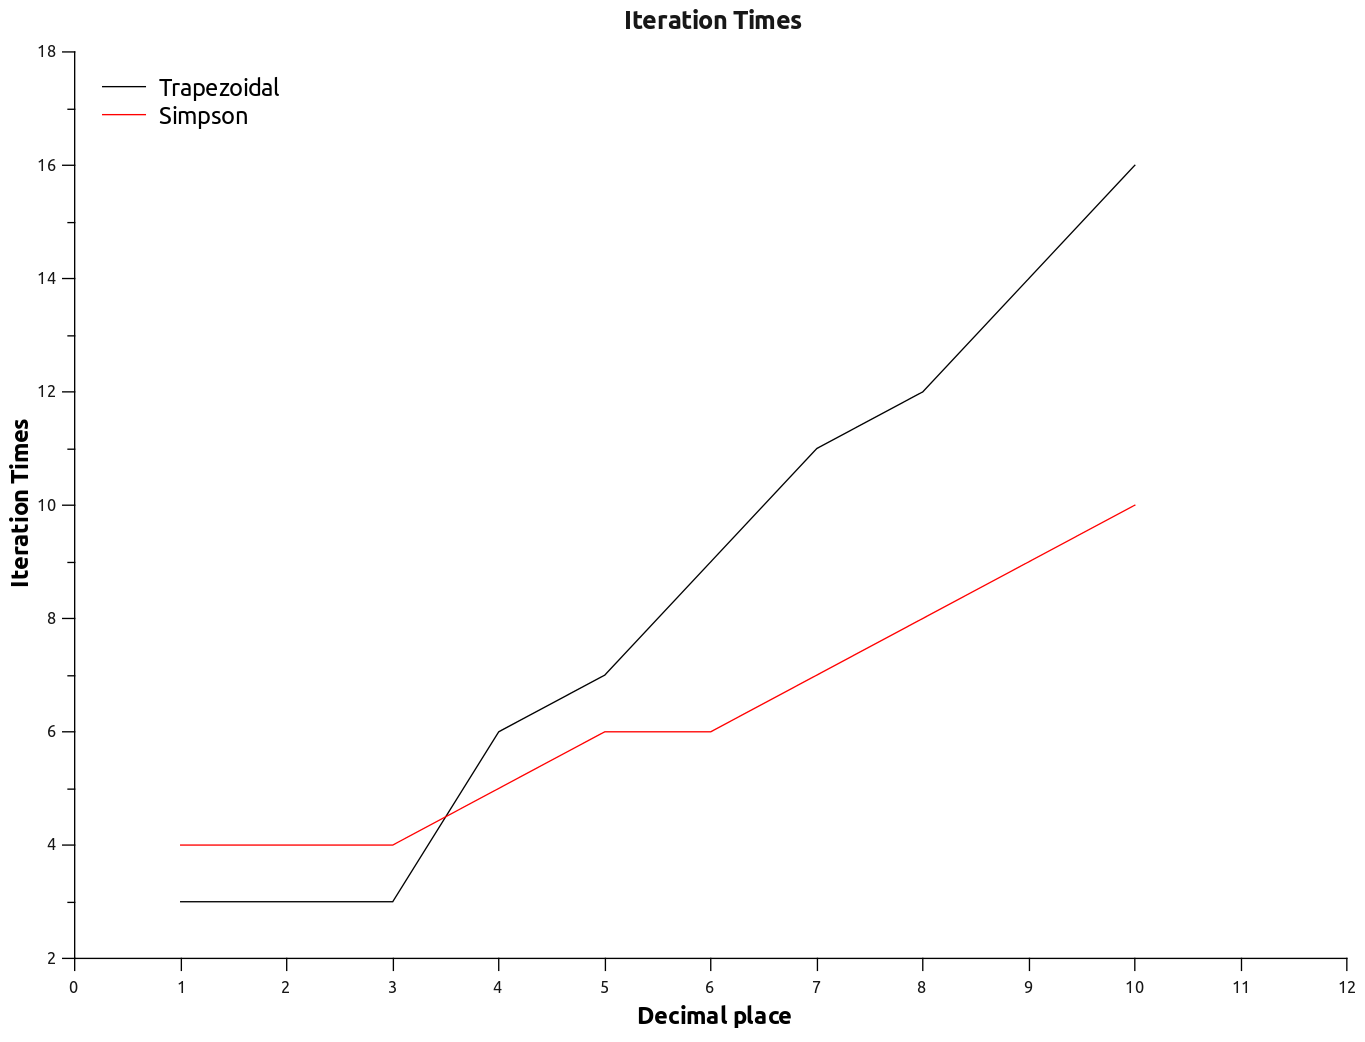
\includegraphics[width=0.8\textwidth]{../result/Graph1.png}
\caption{Simpson法和梯形法收敛速度比较. 横坐标表示精确到的小数点后位数,纵坐标表示迭代次数. 对于i次迭代,需要将[-A,A]区间分$2^i$个区间. 例如要求精确到小数点后10位时,Simpson法需要将区间划分为1024($2^{10}$)个区间,而梯形法需要65536($2^{16}$)个区间才能收敛到同样的精度.}
\end{figure}
\end{document}